\documentclass{scrartcl}
\usepackage{lipsum}
%%\usepackage[french]{babel}
%%\usepackage[ngerman]{babel}


%% Choose default font for the document
%% Warning : only ONE of the following should be enabled
\usepackage{kpfonts}
%%\usepackage{libertine}

%% The following chose the default language for the document and
%% use the default typography rules for the choosen language.
\usepackage{polyglossia}
\setdefaultlanguage{english}
%% \setdefaultlanguage{german}
%%\setdefaultlanguage{french}

\usepackage[backend=biber, style=ieee]{biblatex}
\addbibresource{template.bib}

\usepackage{graphicx}
\graphicspath{ {./ressources/images} }

\usepackage{array}

\usepackage{listings}

\begin{document}
\title{Web Simulation of a Thymio Robot}
\date{\today}   %% or \date{01 november 2018}
\author{Quentin Flückiger (\texttt{flucq1@bfh.ch})}

\clearpage
\maketitle
\tableofcontents
\clearpage

\section{Introduction}

\section{Environment}

\subsection{Thymio}
\subsubsection{What is Thymio} 

Thymio is an educational robot that aims at improving early education (starting in primary school) in STEM (Science, Technology, Engineering and Mathematics), computational thinking, base computer science and researching the acknowledgment by kids of robots in their learning environment. The project also had technical aims, such as how to provide hardware modularity, fast reaction time amid perception and action, clear internal communication bus in a user-friendly way and streamline development for group robot, this includes direct changes to the robots’ programs and parallel debugging wirelessly, transparently and cheaply.
The Thymio project is based on a collaboration between the MOBOTS group from the Swiss Federal Institute of Technology in Lausanne (EPFL) and the Lausanne Arts School (ECAL). MOBOTS being the Miniature Mobile Robots Group, they are mainly focused around system design for small robots of the kind. It started with a strange-looking pile of components, that were assembled on any kind of support and holt the name of “Monsieur Patate” (Sir Potato), most likely due to its appearance, that saw life during the first workshop between the two contributors. After what the first “Thymio” was developed, it was a four-block robot that could be self-assembled, but not self-programmed as it was coming with pre-programmed behaviours. It was used as a user study to gather feedback from clients to know what features needed to be implemented on the Thymio II.
\begin{figure}[h!]
  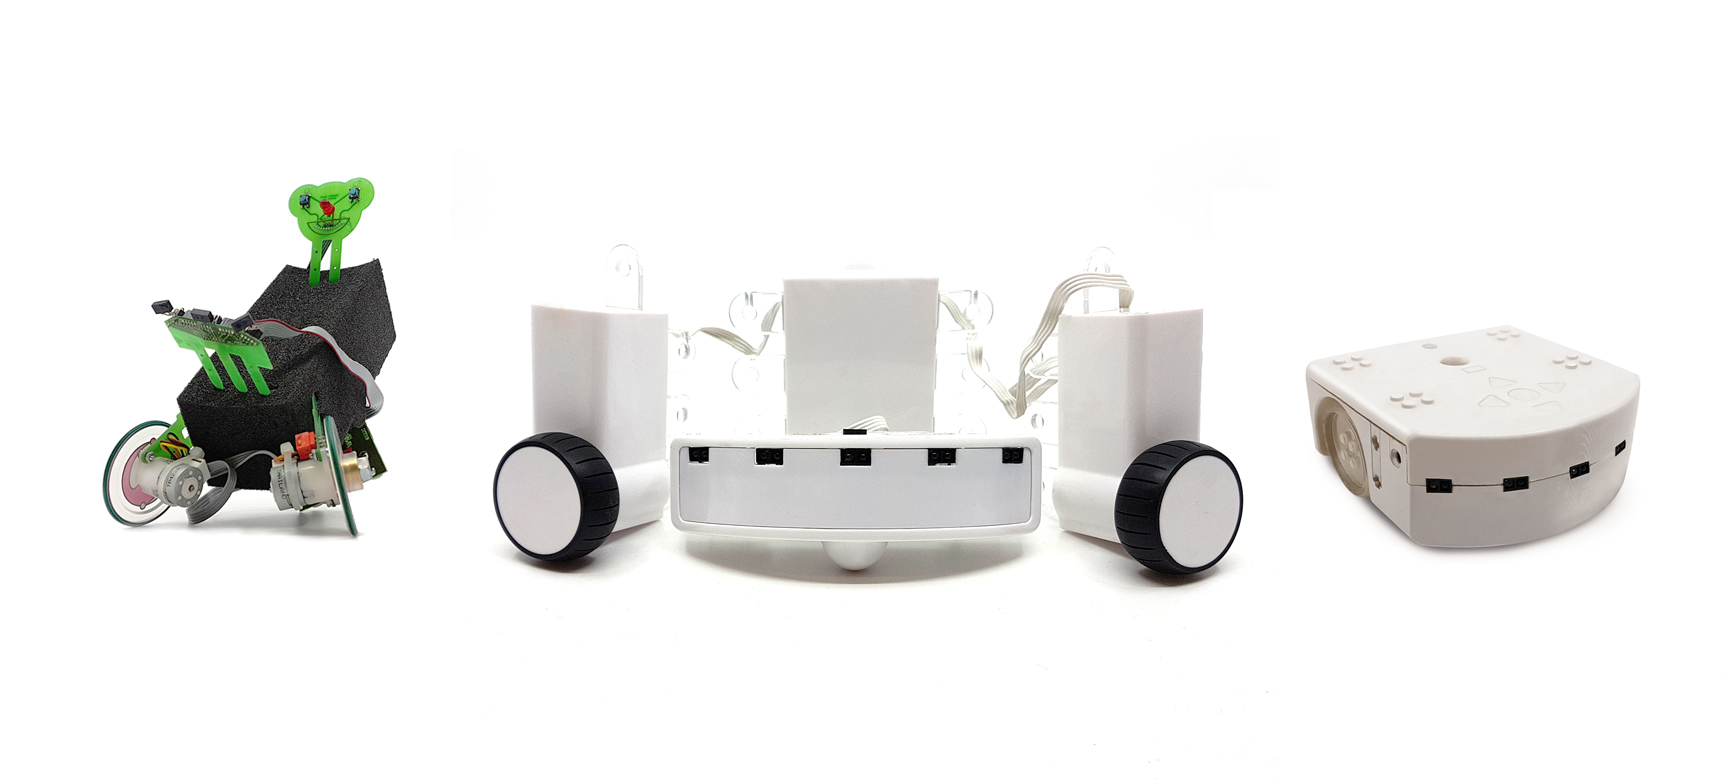
\includegraphics[width=\textwidth]{prototype_thymio_old}
  \caption{From left to right, "Monsieur Patate", Thymio, Thymio II}
  \label{fig:thymio_prototype}
\end{figure}

\subsubsection{How does it works}
\subsubsection{The different programming languages}
\paragraph{VPL}
\paragraph{Blockly}
\paragraph{Scratch}
\paragraph{Aseba}
\subsubsection{What already exist} 

\subsection{TypeScript}
\subsection{Three JS}

For that we red the article book of \cite{Jerald:2015:VBH:2792790}
which is very interesting, much more than the article
\cite{Diniz:2017:UGO:3100317.3100324}

\section{Conclusion and future work}

\section{Appendices}
\subsection{Virtual Machine Configuration}
Step by step Guide on how to set it up and use it.
\subsection{Mettings}
\begin{tabular}{ | m{3cm} | m{10cm} | }
  \hline
  Date & Content \\
  \hline
  17.09.2019 & \textbf{Kick Off meeting}\\
  & Documentation/Management\\
  & Technology to use : ThreeJS and Typescript\\
  & Setting up the goals\\
  \hline
  24.09.2019 & \textbf{Second meeting} \\
  & Documentation language : English \\
  & Thymio model \\
  & Base talk about riks management \\
  \hline
\end{tabular}



%% Print the bibibliography and add the section to the table of content
\printbibliography[heading=bibintoc]

\end{document}
